\begin{figure*}[h!]
    \centering

    \subfloat[Input]{
        \includegraphics[width=0.11\linewidth]{figs/SR/LR}
    }
    \subfloat[Ground Truth]{
        \includegraphics[width=0.11\linewidth]{figs/SR/HR}
    }
    \subfloat[MAE]{
        \includegraphics[width=0.11\linewidth]{figs/SR/Ours@Residual@L1}
    }
    \subfloat[MSE]{
        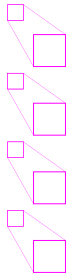
\includegraphics[width=0.11\linewidth]{figs/SR/Ours@Residual@L2}
        \label{figure:comparisons/large/mse}
    }
    \subfloat[SSIM]{
        \includegraphics[width=0.11\linewidth]{figs/SR/Ours@Residual@SSIM}
    }
    \subfloat[MS-SSIM]{
        \includegraphics[width=0.11\linewidth]{figs/SR/Ours@Residual@MS-SSIM}
    }
    \subfloat[Perceptual]{
        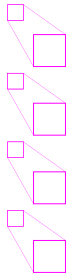
\includegraphics[width=0.11\linewidth]{figs/SR/Ours@Residual@Perceptual}
    }
    \subfloat[MixGE]{
        \includegraphics[width=0.11\linewidth]{figs/SR/Ours@Residual@Sobel}
    }
    \caption{
        Comparison across loss functions on our \textbf{Large} network. See Figure~\ref{figure:comparisons} for image sources.
    }

    \label{figure:comparisons-large}
\end{figure*}
